
\documentclass[conference]{IEEEtran}
% Some Computer Society conferences also require the compsoc mode option,
% but others use the standard conference format.
%
% If IEEEtran.cls has not been installed into the LaTeX system files,
% manually specify the path to it like:
% \documentclass[conference]{../sty/IEEEtran}

% *** GRAPHICS RELATED PACKAGES ***
%
\ifCLASSINFOpdf
  \usepackage[pdftex]{graphicx}
  % declare the path(s) where your graphic files are
  % \graphicspath{{../pdf/}{../jpeg/}}
  % and their extensions so you won't have to specify these with
  % every instance of \includegraphics
  % \DeclareGraphicsExtensions{.pdf,.jpeg,.png}
\else
  % or other class option (dvipsone, dvipdf, if not using dvips). graphicx
  % will default to the driver specified in the system graphics.cfg if no
  % driver is specified.
  % \usepackage[dvips]{graphicx}
  % declare the path(s) where your graphic files are
  % \graphicspath{{../eps/}}
  % and their extensions so you won't have to specify these with
  % every instance of \includegraphics
  % \DeclareGraphicsExtensions{.eps}
\fi
% graphicx was written by David Carlisle and Sebastian Rahtz. It is
% required if you want graphics, photos, etc. graphicx.sty is already
% installed on most LaTeX systems. The latest version and documentation
% can be obtained at: 
% http://www.ctan.org/pkg/graphicx
% Another good source of documentation is "Using Imported Graphics in
% LaTeX2e" by Keith Reckdahl which can be found at:
% http://www.ctan.org/pkg/epslatex
%
% latex, and pdflatex in dvi mode, support graphics in encapsulated
% postscript (.eps) format. pdflatex in pdf mode supports graphics
% in .pdf, .jpeg, .png and .mps (metapost) formats. Users should ensure
% that all non-photo figures use a vector format (.eps, .pdf, .mps) and
% not a bitmapped formats (.jpeg, .png). The IEEE frowns on bitmapped formats
% which can result in "jaggedy"/blurry rendering of lines and letters as
% well as large increases in file sizes.
%
% You can find documentation about the pdfTeX application at:
% http://www.tug.org/applications/pdftex


% correct bad hyphenation here
\hyphenation{op-tical net-works semi-conduc-tor}


\usepackage{adjustbox}  
\usepackage{amsmath}

\begin{document}
%
% paper title
% Titles are generally capitalized except for words such as a, an, and, as,
% at, but, by, for, in, nor, of, on, or, the, to and up, which are usually
% not capitalized unless they are the first or last word of the title.
% Linebreaks \\ can be used within to get better formatting as desired.
% Do not put math or special symbols in the title.
\title{Image-based segmentation and localization of surgical instruments using deep neural networks}


% author names and affiliations
% use a multiple column layout for up to three different
% affiliations
\author{\IEEEauthorblockN{Amelie Wagner}
%\IEEEauthorblockA{School of Electrical and\\Computer Engineering\\
%Georgia Institute of Technology\\
%Atlanta, Georgia 30332--0250\\
%Email: http://www.michaelshell.org/contact.html}
}

% use for special paper notices
%\IEEEspecialpapernotice{(Invited Paper)}



% make the title area
\maketitle

% As a general rule, do not put math, special symbols or citations
% in the abstract
\begin{abstract}
Segmentation and localization of surgical instruments in endoscopic videos during minimally invasive surgery is a current challenge for evaluating and supporting the performance of the surgeon. 

For the instrument segmentation task, every pixel of the input image has to be labeled as background or instrument.
For the instrument localization task, the position of the instrument center point in the image has to be estimated.
For the instrument segmentation task, every pixel of the network input image is labeled as black for background or white for instrument.
In this work, both tasks are solved jointly by an adjusted TernausNet-11 network. For the localization task, the TernausNet-11 predicts a heatmap centered at the position of the instrument center point.
Afterwards, the center point coordinates of each instrument are extracted by using weighted k-means clustering. Every model proposed in this work is evaluated on the robotic dataset of the MICCAI 2015 Endoscopic Vision, on the subchallenge instrument segmentation and tracking according to the challenge guidelines. The evaluation results show that the proposed method is able to solve both tasks on the same level as state-of-the-art methods.
\end{abstract}

% no keywords

% For peer review papers, you can put extra information on the cover
% page as needed:
% \ifCLASSOPTIONpeerreview
% \begin{center} \bfseries EDICS Category: 3-BBND \end{center}
% \fi
%
% For peerreview papers, this IEEEtran command inserts a page break and
% creates the second title. It will be ignored for other modes.
\IEEEpeerreviewmaketitle


\section{Introduction}
Minimally invasive surgery (MIS) is a surgical technique that has several advantages in comparison to the commonly used standard open approach, for example shorter recovery time and hospital stays after the intervention~\cite{laparoscp2002lacy}. %~\cite{laparoscopic_adrenalectomy1996rutherford}. 
Because the field of view for the surgeon is reduced by the endoscopic camera and the instruments can only be seen two-dimensional, it is important to support the surgeon during this procedure~\cite{detect_instruments_mis2013allan}. Segmenting and locating the instruments directly out of the endoscopic video images is an attractive possibility for this, especially because no modification of the surgical scene is required. 
The goal of this work is the segmentation and localization of surgical instruments out of endoscopic video images. For the segmentation task, the image is partitioned into black pixels for background and white pixels for instrument. For the localization task, the coordinates of the instrument center point are extracted out of the image. 
In this work, a Convolutional Neural Network (CNN) is used for segmenting and localizing the instrument. It is based on \mbox{TernausNet-11}~\cite{Shvets2018} that already solves the segmentation task. The resulting localization network is able to solve the localization task based on the information learned for segmentation. % This method was recently proposed by Laina et al.~\cite{Laina2017}. 


\section{Methods}

\subsection{Instrument Localization Network} 
The segmentation network TernausNet-11 is extended by three more layers to solve the localization task. It predicts two outputs, one for the segmentation and one for the localization task. 
The output of the segmentation output layer is a binary image, that contains a white segmentation mask
where the instrument is located. 
The output for the localization task is a greyscale heatmap. A high pixel
value at the predicted heatmap indicates a high probability that the instrument center point is located at this pixel position. The network is abbreviated as~\emph{LocNet}. %maybe example pic reference here 

\subsection{Heatmaps}
It is necessary to convert the localization targets, given as two-dimensional image positions,
into greyscale images, in order to make it possible for LocNet to process them. The heatmaps are generated by calculating a two-dimensional Gaussian distribution
$gauss2D(x_r,y_r)$, centered at the center point $(x_{cp}, y_{cp})$ of the instrument.

\begin{equation}
\label{eq:gauss2D_function}
H(x_r,y_r)=gauss2D(x_r,y_r) = \frac{1}{\sqrt{2\pi\sigma^2} } e^{ -\frac{(x_r-x_{cp})^2 + (y_r-y_{cp})^2}{2\sigma^2} }
\end{equation}

The standard deviation $\sigma$ controls the spread of the Gaussian around the instrument
location. $\sigma^2$ denotes the variance.
By iterating over the dimensions of the training input image and applying $gauss2D(x_r,y_r)$, a heatmap with the same dimensions is generated out of the ground truth instrument position.
$(x_r, y_r)$ is one pixel position of the training image, which corresponds to the pixel position in the generated heatmap.
% following sentences: maybe unnecessary
When two instruments are visible in the input image, the heatmap is generated by calculating two Gaussian distributions, one for each instrument % insert ref to image with 2 instruments?


\section{Postprocessing}
The heatmaps predicted by the network mostly have a pixel range from $[127,255]$.
In order to improve the extraction of the instrument position, the pixel values of the predicted heatmaps are thresholded with $threshold$ set to 129:

\[
    thresh(H(x_r,y_r))= 
\begin{cases}
    H(x_r,y_r)& \text{if } H(x_r,y_r)\geq threshold\\
    0         & \text{otherwise}
\end{cases}
\]

In a second postprocessing step, histogram equalization~\cite{equalization_histogram1987pizer} is used to increase the contrast of the Gaussian distribution in the image.

To get the instrument position out of the thresholded heatmap, \emph{k-means} clustering is used. It is a commonly used method to automatically partition a dataset into $k$ groups~\cite{k-means-paper2005sipkins}.
When the input to the corresponding predicted heatmap contains one instrument, $k$ is set to 1. When two instruments are visible in the input image, $k$ is set to 2.
The pixel values of the thresholded heatmap are used as weights for the k-means clustering to improve the results, because a higher pixel value indicates a higher probability that the instrument center point is located at that position.

\section{Evaluation}
\subsection{Endoscopic Vision Challenge 2015}
The datasets used for segmentation and localization are proposed in the subchallenge Instrument Segmentation and Tracking of the MICCAI Endoscopic Vision Challenge 2015~\cite{EndoVis15}. The subchallenge is abbreviated as \emph{EndoVis15}.
The robotic set of the subchallenge that is used in this work, is separated in a segmentation and a localization part.
% the instruments show typical poses and articulation in robotic surgery.  There is some occlusion, but no smoke and bleeding in any sequence.
One input image has two different ground truth annotations, one for each subchallenge part.
The segmentation part is abbreviated as \emph{EndoVis15-S}, the tracking part is abbreviated as \emph{EndoVis15-T}. % insert references for example pics

\begin{figure}%[!t]
\centering
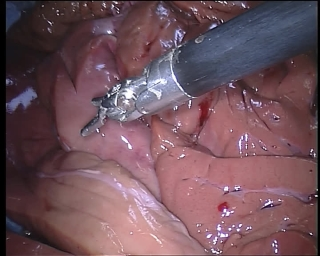
\includegraphics[width=0.6\linewidth]{../images/dataset/robotic15_segm/image_frame001-1instrument.jpg}
% 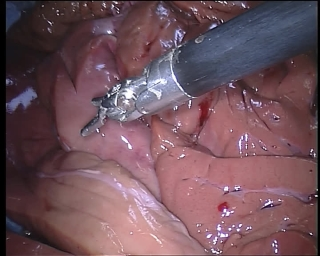
\includegraphics[width=2.5in]{../images/dataset/robotic15_segm/image_frame001-1instrument.jpg}
\caption{Example image out of Endoscopic Vision Challenge 2015.}
\label{img:endo_vis15_example_frame_orig}
\end{figure}

\begin{figure}%[!t]
\centering
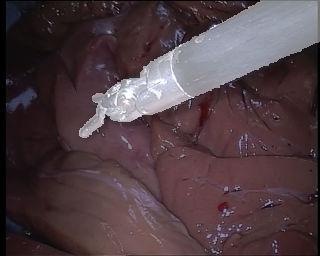
\includegraphics[width=0.6\linewidth]{../images/dataset/robotic15_segm/frame001_dataset2_superimposed_mask-.png}
% 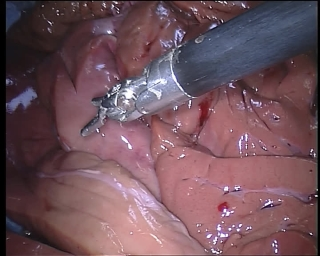
\includegraphics[width=2.5in]{../images/dataset/robotic15_segm/image_frame001-1instrument.jpg}
\caption{Example image out of Endoscopic Vision Challenge 2015 with superimposed segmentation mask.}
\label{img:endo_vis15_example_frame_mask}
\end{figure}

\begin{figure}%[!t]
\centering
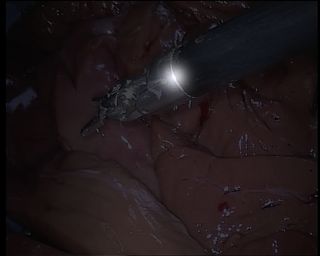
\includegraphics[width=0.6\linewidth]{../images/dataset/robotic15_segm/img+heatmap_1instrument.png}
% 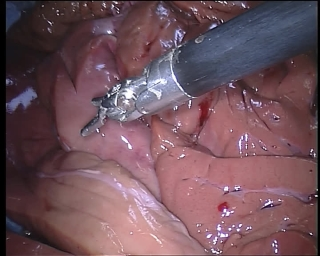
\includegraphics[width=2.5in]{../images/dataset/robotic15_segm/image_frame001-1instrument.jpg}
\caption{Example image out of Endoscopic Vision Challenge 2015 with superimposed heatmap.}
\label{img:endo_vis15_example_frame_heatmap}
\end{figure}


\subsection{Experiments}
% include result tables somehow beautiful (only necessary tables: localization 
% bzw.: nur beste 2 netze LOSO und T4 -> dann aber nochmal LOSO und T4 erklären
After preprocessing the proposed datasets, LocNet was
trained and evaluated in different ways with the \mbox{EndoVis-15}
datasets. Each model is trained and evaluated according to one of the EndoVis15 challenge guidelines: On each of the four surgeries, one model one model is evaluated that has been trained on the remaining three surgeries (LOSO). The other evaluation method consists of training on all train sets and then testing on the test sets (T4).
The results of the best models for each evaluation method are proposed in table~\ref{tab:loc_results_datasets_LOSO} and table~\ref{tab:loc_results_datasets_T4}.
The models were trained to the conditions stated in table~\ref{tab:training_descr_locnet}.


\begin{table}
\begin{adjustbox}{center=\linewidth}
\begin{tabular}{c c c c c}
\hline\noalign{\smallskip}
\multicolumn{5}{c}{\textbf{Best Localization Results LOSO}} \\
Dataset1 left/right instr. & Dataset2 & Dataset3 & Dataset4 & mean dist.\\
\hline\noalign{\smallskip}
$17.58/ 15.15$ & $11.36$ & $10.83$ & $12.05$ & $13.85$ \\ [0.5ex] 
\end{tabular}
\end{adjustbox}
\caption[LocNet results LOSO]{Results for the different datasets for the best LOSO LocNet model.
Mean dist. is the mean distance over all datasets. Dataset1 is distinguished into left and right instrument (left/right instr.).
The evaluation results are given as mean value over all prediction results. The distance between ground truth location and predicted location of the instrument is given in pixels.}
\label{tab:loc_results_datasets_LOSO}
\end{table}

\begin{table}
\begin{tabular}{c c c}
\hline\noalign{\smallskip}
\multicolumn{3}{c}{\textbf{Localization Results Datasets T4}} \\
Dataset5 left/right instr.& Dataset6 left/right instr.& mean dist.\\
 \hline\noalign{\smallskip}
 $89.80/ 117.91 $ & $88.17 / 120.02$ & $106.4$\\ [0.5ex]
\end{tabular}
\caption[LocNet results tests EndoVis15-T]{Results of the best T4 LocNet model. %T4 denotes that the models were trained completely on the four training sets and tested on the two test sets.
Each dataset is distinguished into left and right instrument (left/right instr.).
Mean dist. is the mean distance over all datasets. The evaluation results are given as mean value over all prediction results $\pm$ the standard deviation. The distance between ground truth location and predicted location of the instrument is given in pixels.}
\label{tab:loc_results_datasets_T4}
\end{table}

\begin{table}
\centering
 \begin{tabular}{l c c } 
 \hline\noalign{\smallskip}
 \multicolumn{3}{c}{\textbf{Training Conditions LocNet}} \\
	val. method & epochs & $\gamma$  \\ [0.5ex]
 \hline \noalign{\smallskip}
 LOSO model & 50 & $1/2$ \\ 
 T4 model & 500 & $1/2$ \\ [0.5ex]
  \end{tabular}  
\caption[LocNet training conditions]{Validation method (val.method) specifies if the model was trained according to the LOSO fashion (LOSO), or trained completely on the four training sets and tested on the two test sets (T4). The impact of the segmentation and the localization loss on the model is adjusted by $\gamma$.}
\label{tab:training_descr_locnet}
\end{table}

\section{Conclusion}
The achieved results are comparable to other state-of-the-art approaches.
% future work section:
Besides taking further postprocessing steps to improve results, the proposed method could be combined with a temporal tracking algorithm. In this case, the estimated instrument locations could serve as input to trackers such as Kalman filter or Particle filter~\cite{kalman_filter1992brown}. Temporal tracking would be especially helpful to deal with occlusions and to associate each heatmap with either the left or the right instrument, even when instruments cross.

\bibliographystyle{IEEEtran}

\bibliography{bibliography}

\end{document}


% *** SUBFIGURE PACKAGES ***
%\ifCLASSOPTIONcompsoc
%  \usepackage[caption=false,font=normalsize,labelfont=sf,textfont=sf]{subfig}
%\else
%  \usepackage[caption=false,font=footnotesize]{subfig}
%\fi
% subfig.sty, written by Steven Douglas Cochran, is the modern replacement
% for subfigure.sty, the latter of which is no longer maintained and is
% incompatible with some LaTeX packages including fixltx2e. However,
% subfig.sty requires and automatically loads Axel Sommerfeldt's caption.sty
% which will override IEEEtran.cls' handling of captions and this will result
% in non-IEEE style figure/table captions. To prevent this problem, be sure
% and invoke subfig.sty's "caption=false" package option (available since
% subfig.sty version 1.3, 2005/06/28) as this is will preserve IEEEtran.cls
% handling of captions.
% Note that the Computer Society format requires a larger sans serif font
% than the serif footnote size font used in traditional IEEE formatting
% and thus the need to invoke different subfig.sty package options depending
% on whether compsoc mode has been enabled.
%
% The latest version and documentation of subfig.sty can be obtained at:
% http://www.ctan.org/pkg/subfig



% An example of a double column floating figure using two subfigures.
% (The subfig.sty package must be loaded for this to work.)
% The subfigure \label commands are set within each subfloat command,
% and the \label for the overall figure must come after \caption.
% \hfil is used as a separator to get equal spacing.
% Watch out that the combined width of all the subfigures on a 
% line do not exceed the text width or a line break will occur.
%
%\begin{figure*}[!t]
%\centering
%\subfloat[Case I]{\includegraphics[width=2.5in]{box}%
%\label{fig_first_case}}
%\hfil
%\subfloat[Case II]{\includegraphics[width=2.5in]{box}%
%\label{fig_second_case}}
%\caption{Simulation results for the network.}
%\label{fig_sim}
%\end{figure*}
%
% Note that often IEEE papers with subfigures do not employ subfigure
% captions (using the optional argument to \subfloat[]), but instead will
% reference/describe all of them (a), (b), etc., within the main caption.
% Be aware that for subfig.sty to generate the (a), (b), etc., subfigure
% labels, the optional argument to \subfloat must be present. If a
% subcaption is not desired, just leave its contents blank,
% e.g., \subfloat[].



% *** CITATION PACKAGES ***
%
%\usepackage{cite}
% cite.sty was written by Donald Arseneau
% V1.6 and later of IEEEtran pre-defines the format of the cite.sty package
% \cite{} output to follow that of the IEEE. Loading the cite package will
% result in citation numbers being automatically sorted and properly
% "compressed/ranged". e.g., [1], [9], [2], [7], [5], [6] without using
% cite.sty will become [1], [2], [5]--[7], [9] using cite.sty. cite.sty's
% \cite will automatically add leading space, if needed. Use cite.sty's
% noadjust option (cite.sty V3.8 and later) if you want to turn this off
% such as if a citation ever needs to be enclosed in parenthesis.
% cite.sty is already installed on most LaTeX systems. Be sure and use
% version 5.0 (2009-03-20) and later if using hyperref.sty.
% The latest version can be obtained at:
% http://www.ctan.org/pkg/cite
% The documentation is contained in the cite.sty file itself.

% *** MATH PACKAGES ***
%
%\usepackage{amsmath}
% A popular package from the American Mathematical Society that provides
% many useful and powerful commands for dealing with mathematics.
%
% Note that the amsmath package sets \interdisplaylinepenalty to 10000
% thus preventing page breaks from occurring within multiline equations. Use:
%\interdisplaylinepenalty=2500
% after loading amsmath to restore such page breaks as IEEEtran.cls normally
% does. amsmath.sty is already installed on most LaTeX systems. The latest
% version and documentation can be obtained at:
% http://www.ctan.org/pkg/amsmath
